\documentclass[14pt]{extarticle}
% \documentclass[14pt]{article}

% \usepackage[style=authoryear,maxbibnames=9,maxcitenames=2,uniquelist=false,backend=biber,doi=false,url=false]{biblatex}
% \addbibresource{$BIB} % bibtex location
% \renewcommand*{\nameyeardelim}{\addcomma\space} % have comma in parencite
\usepackage{natbib}

\usepackage{xcolor}
\usepackage{amsmath}
\newcommand{\tuple}[1]{ \langle #1 \rangle }
%\usepackage{automata}
\usepackage{times}
\usepackage{ltablex}
\usepackage{tasks}

%%%%%% Template
\usepackage{hyperref}
\hypersetup{colorlinks=true,allcolors=blue}

\usepackage{vmargin}
\setpapersize{USletter}
\setmarginsrb{1.0in}{1.0in}{1.0in}{0.6in}{0pt}{0pt}{0pt}{0.4in}

% HOW TO USE THE ABOVE:
%\setmarginsrb{leftmargin}{topmargin}{rightmargin}{bottommargin}{headheight}{headsep}{footheight}{footskip}
%\raggedbottom
% paragraphs indent & skip:
\parindent  0.3cm
\parskip    -0.01cm

\usepackage{tikz}
\usetikzlibrary{backgrounds}

% hyphenation:
% \hyphenpenalty=10000 % no hyphen
% \exhyphenpenalty=10000 % no hyphen
\sloppy

% notes-style paragraph spacing and indentation:
\usepackage{parskip}
\setlength{\parindent}{0cm}

% let derivations break across pages
\allowdisplaybreaks

\newcommand{\orange}[1]{\textcolor{orange}{#1}}
\newcommand{\blue}[1]{\textcolor{blue}{#1}}
\newcommand{\red}[1]{\textcolor{red}{#1}}
\newcommand{\freq}[1]{{\bf \sf F}(#1)}
\newcommand{\datafreq}[2]{{{\bf \sf F}_{#1}(#2)}}

\def\qqquad{\quad\qquad}
\def\qqqquad{\qquad\qquad}

%%%%%%%%%%%%%%%%%%%%%%%%%%%%%%%%%%%%%%%%%%%%%%%%%%%%%%%%%%%%%%%%%%%%%%%%%%%%%%%%
%%%%%%%%%%%%%%%%%%%%%%%%%%%%%%%%%%%%%%%%%%%%%%%%%%%%%%%%%%%%%%%%%%%%%%%%%%%%%%%%

% fill-in-blank question style, found in https://tex.stackexchange.com/a/505089

\usepackage{ifthen}
\usepackage{tocloft}
\usepackage{exercise}
% \usepackage{xcolor}

% Set the Show Answers Boolean
\newboolean{showAns}
\setboolean{showAns}{false}
\newcommand{\showAns}{\setboolean{showAns}{true}}

% The length of the Answer line
\newlength{\answerlength}
\newcommand{\anslen}[1]{\settowidth{\answerlength}{#1}}

% ans command that indicates space for an answer or shows the answer in red
\newcommand{\ans}[1]{\settowidth{\answerlength}{\hspace{2ex}#1\hspace{2ex}}%
    \ifthenelse{\boolean{showAns}}%
        {\textcolor{red}{\underline{\hspace{2ex}#1\hspace{2ex}}}}%
        {\underline{\hspace{\answerlength}}}}%

\newcommand{\details}[1]{\settowidth{\answerlength}{#1}%
    \ifthenelse{\boolean{showAns}}%
        {\\ \textcolor{blue}{#1}}%
        {}}%

% Formatting how multiple choices Questions are formated.
\settasks{label=(\Alph*), label-width=30pt}


% Some commands for the Exercise Question package
\renewcommand{\QuestionNB}{\Large\protect\textcircled{\small\bfseries\arabic{Question}}\ }
\renewcommand{\ExerciseHeader}{} %no header
\renewcommand{\QuestionBefore}{3ex} %Space above each Q
\setlength{\QuestionIndent}{8pt} % Indent after Q number


% To create the list of answers with tocloft...
\newcommand{\listanswername}{Answers}
\newlistof[Question]{answer}{Answers}{\listanswername}

% Creates a TOC for Answers
\newcounter{prevQ}
\newcommand{\answer}[1]{\refstepcounter{answer}%
\ans{#1}%
\ifnum\theQuestion=\theprevQ%
        \addcontentsline{Answers}{answer}{\protect\numberline{}#1}% don't include the Q number
        \else%
        \addcontentsline{Answers}{answer}{\protect\numberline{\theQuestion}#1}%
        \setcounter{prevQ}{\value{Question}}%
        \fi%
        }%

% \hyphenpenalty=10000 % no hyphen
% \exhyphenpenalty=10000 % no hyphen
\sloppy              % hyphen

\newcommand{\HRule}{\rule{\linewidth}{0.5mm}}
\newcommand{\Hrule}{\rule{\linewidth}{0.3mm}}

%tocloft formatting listofanswers
\renewcommand{\cftAnswerstitlefont}{\bfseries\large}
\renewcommand{\cftanswerdotsep}{\cftnodots}
\cftpagenumbersoff{answer}
\addtolength{\cftanswernumwidth}{10pt}

\makeatletter% since there's an at-sign (@) in the command name
\renewcommand{\@maketitle}{%
  \parindent=0pt% don't indent paragraphs in the title block
  \centering
  {\Large \bfseries\textsc{\@title}} \\
  \vspace{5pt}
  {\large \textit{\@author}} \\
  \HRule \\
  \vspace{1em}
}
\makeatother% resets the meaning of the at-sign (@)

\title{ECON 2002.01 Problem Set 10}
\author{Unit 16 \\
  \vspace{5pt}
    Hui-Jun Chen}


%%%%%%%%%%%%%%%%%%%%%%%%%%%%%%%%%%%%%%%%%%%%%%%%%%%%%%%%%%%%%%%%%%%%%%%%%%%%%%%%
%%%%%%%%%%%%%%%%%%%%%%%%%%%%%%%%%%%%%%%%%%%%%%%%%%%%%%%%%%%%%%%%%%%%%%%%%%%%%%%%
\begin{document}

\maketitle

\showAns
\listofanswer

    % 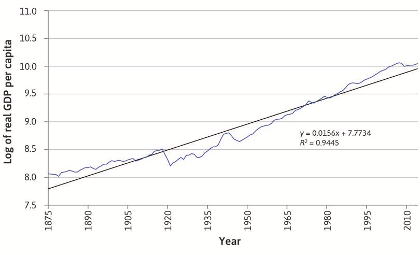
\includegraphics[width=\textwidth]{../QuestionBankImage/OUP-U13-Q04-01.png}

\begin{Exercise}




\Question (OUP-U16-Q4)
In the short run, successive additions to capital produce smaller and smaller increases in output. Which of the following statement(s) could explain why GDP nevertheless continues to rise In the long run?
\answer{D}
\begin{tasks}(1)
    \task Workers work harder.
        \details{Incorrect. Worker effort is not directly related to the state of technology. Equipping workers with the latest technology may raise their morale and encourage them to work harder if they see the new technology as a vote of confidence from the firms’ owners. On the other hand, knowing that the new technology makes them more productive, they may be tempted to work less hard in order to produce the same as before.}
    \task Government policy encourages economic growth.
        \details{Incorrect. Generally speaking, governments tend to favour economic growth. But the mere fact that governments prefer growth to stagnation does not make it happen.}
    \task Economies benefit from economies of scale.
        \details{Incorrect. Individual firms may enjoy economies of scale, meaning that the unit cost of production falls as output increases. But true economies of scale must come solely from increasing the volume of production. Everything else, including the capital stock, should remain constant.}
    \task New capital equipment incorporates the latest technological developments.
        \details{Correct. In the short run, the additions to capital consist of the same kind of equipment as earlier additions to the capital stock. Eventually, ‘more of the same’ type may still increase the level of output, but at a diminishing rate. But once we relax the short-run constraint, successive additions to capital cease to be ‘more of the same’ and rather will consist of more and more productive equipment.}
\end{tasks}



\Question (OUP-U16-Q8)
The relationship between the unemployment rate and the job vacancy rate (each expressed as a fraction of the labour force) is known as:
\answer{D}
\begin{tasks}(1)
    \task The Phillips curve.
        \details{Incorrect. The Phillips curve plots the rate of growth of wages against the level of unemployment.}
    \task The labour demand curve.
        \details{Incorrect. The labour demand curve shows the quantity of labour demanded (by employers) at each level of real wages.}
    \task The wage-setting curve.
        \details{Incorrect. The wage-setting curve shows the amount of labour that workers are willing to supply at each level of real wages.}
    \task The Beveridge curve.
        \details{Correct. The Beveridge curve shows the relationship between the unemployment rate and the job vacancy rate.}
\end{tasks}




\Question (OUP-U16-Q11)
The profit-maximising mark-up declines as the number of firms increases. This is because:
\answer{D}
\begin{tasks}(1)
    \task The greater the number of firms, the more market power they each have.
        \details{Incorrect. The greater the number of firms, the less market power any one firm is likely to have.}
    \task Too many firms means diseconomies of scale.
        \details{Incorrect: Economies or diseconomies of scale occur within an individual firm. It has nothing to do with the number of firms.}
    \task The lower the individual mark-up, the more firms can share in the profits.
        \details{Incorrect. This would be true if the total amount of profit was fixed, but the total amount of profit is likely to vary positively with the number of firms.}
    \task The larger the number of firms, the more competitive the system is likely to be.
        \details{Correct. The larger the number of firms, the more competitive the system is likely to be, and each firm will be obliged to accept the minimum level of profit necessary to keep it functioning.}
\end{tasks}



\Question (OUP-U16-Q14)
The widespread introduction of new technology into an economy takes time. The length of time between first appearance and general acceptance is known as:
\answer{D}
\begin{tasks}(1)
    \task The innovation lag.
        \details{Incorrect. This is a sensible label that could be used to describe the lag between the development of a new technology and its application, but it is not used for this purpose.}
    \task The time gap.
        \details{Incorrect: The term ‘time gap’ is very widely used to describe the time between two events or developments, but it does not refer specifically to the delay here.}
    \task The knowledge lag.
        \details{Incorrect. This could refer to a number of situations but does not relate specifically to innovation.}
    \task The diffusion gap.
        \details{Correct. The ‘diffusion gap’ refers to the length of time required for a technological innovation to become ‘diffused’ throughout the economy.}
\end{tasks}



\Question (OUP-U16-Q16)
As a result of the diffusion of new technology, in the long run we would normally expect:
\answer{D}
\begin{tasks}(1)
    \task The price-setting curve to shift downwards.
        \details{Incorrect. The new technology increases output per worker. There is no reason to suppose that the share of total output required by firms as profit has changed. Therefore the price-setting curve shifts upwards to maintain the firms’ share of total output.}
    \task The price-setting curve to slope downward more steeply.
        \details{Incorrect. The price-setting curve is a horizontal line showing the real wage that firms are willing to pay in order to deliver the desired profit share (= output per worker – real wage).}
    \task An increase in unemployment.
        \details{Incorrect. There may be some unemployment in the short run if some workers are unable to use the new technology, but the lasting effect depends on what happens to the wage-setting curve. If it remains unchanged, there will be a fall in unemployment, rather than an increase.}
    \task The price-setting curve to shift upwards.
        \details{Correct. The new technology increases output per worker. There is no reason to suppose that the share of total output required by firms as profit has changed. Therefore the price-setting curve shifts upwards to maintain the firms’ share of total output.}
\end{tasks}




\Question (OUP-U16-Q20)
The figure shows long-run unemployment and real wage growth across the OECD. The rays drawn from the origin are described as ‘indifference curves’. This is because:
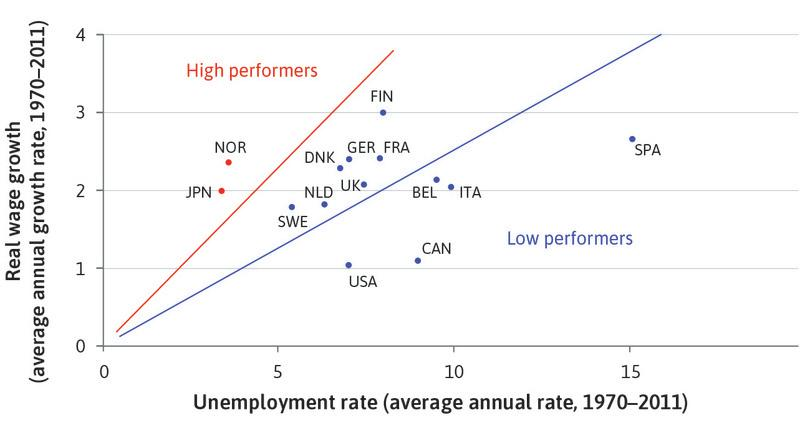
\includegraphics[width=\textwidth]{../QuestionBankImage/OUP-U16-Q20-01.jpg}
\answer{D}
\begin{tasks}(1)
    \task They show that people are indifferent to levels of unemployment.
        \details{Incorrect. ‘Indifferent to levels of unemployment’ would mean that they did not care about the level of unemployment. But an upward-sloping indifference curve means that people are prepared to accept higher unemployment only if real wages grow more rapidly.}
    \task They show a trade-off between unemployment and real wage growth.
        \details{Incorrect. A ‘trade-off’ means that more of something requires less of something else. But here, people are indifferent between combinations of high unemployment and high real wage growth, and low unemployment/low real wage growth. Therefore there is no trade-off involved.}
    \task They show that real wage growth and low unemployment go together.
        \details{`Incorrect. They show that real wage growth and high unemployment go together.}
    \task Each ray shows the combinations of unemployment and real wage growth that correspond to the same 'utility'.
        \details{An indifference curve shows combinations of two variables that give equal satisfaction. In the figure we can see that people can be equally happy with high or low unemployment, provided that higher unemployment is accompanied by higher real wage growth.}
\end{tasks}



\Question (OUP-U16-Q22)
Looking at the figure shown, if it were the case that countries with strong trade unions also experienced high unemployment rates, we would expect the data points to be:
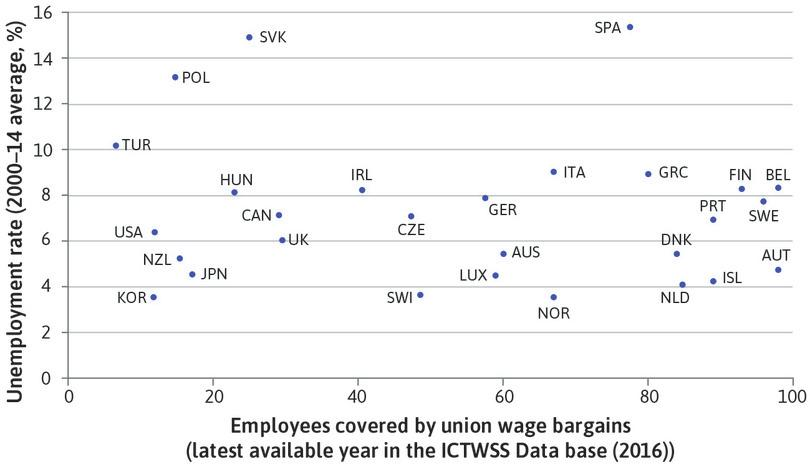
\includegraphics[width=\textwidth]{../QuestionBankImage/OUP-U16-Q22-01.jpg}
\answer{C}
\begin{tasks}(1)
    \task Clustered around a horizontal line.
        \details{Incorrect. If the data points lay close to a horizontal line, this would tell us that the level of unemployment (at which the line were drawn) was consistent with any level of trade union membership. There is no apparent connection between trade union strength and unemployment.}
    \task Clustered around a downward-sloping line.
        \details{Incorrect. If the points were clustered around a downward-sloping line, this would tell us that there might be some connection between unemployment and trade union strength, but the relationship is negative. Trade union strength is associated with low unemployment.}
    \task Clustered around an upward-sloping line.
        \details{Correct. If the points were clustered around an upward-sloping line, this would tell us that there might be some positive connection between unemployment and trade union strength. Trade union strength appears to be linked to high unemployment.}
    \task More randomly dispersed than they are.
        \details{Incorrect. In the figure, the data points are widely dispersed. There is no obvious relation between trade union strength and unemployment. If the data points were more randomly dispersed than they already are, this would make the lack of a connection even clearer.}
\end{tasks}



\Question (OUP-U16-Q9)
The Beveridge curve will shift downward (toward the origin) if:
\answer{C}
\begin{tasks}(1)
    \task Vacancies are increasingly concentrated in given sector of the economy.
        \details{Incorrect. The geographical mismatch of vacancies and workers is one of the reasons why unemployment exists alongside vacancies. If the geographical mismatch increases, there will be more vacancies at each level of unemployment and the Beveridge curve will shift up.}
    \task Vacancies are increasingly concentrated in a geographical region.
        \details{Incorrect. The skills mismatch of vacancies and workers is one of the reasons why unemployment exists alongside vacancies. If the skills mismatch increases, there will be more vacancies at each level of unemployment and the Beveridge curve will shift up.}
    \task Information about job vacancies improves.
        \details{The fact that workers cannot find the matching vacancies and employers cannot find the relevant workers is another reason why vacancies exist alongside unemployment. Helping the two sides to find each other result in more of the vacancies being filled at every level of unemployment, and so the Beveridge curve shifts down.}
    \task Unemployment benefits become more generous.
        \details{Incorrect. An improvement in the availability of unemployment benefits is likely to reduce the efforts put into job search at every level of unemployment. If this happens, the Beveridge curve will shift up.}
\end{tasks}




\Question (ECO-U16-Q7)
Figure 16.9b depicts the long-run adjustment process in the labour market after technological progress. Based on this information, which of the following statements is correct?
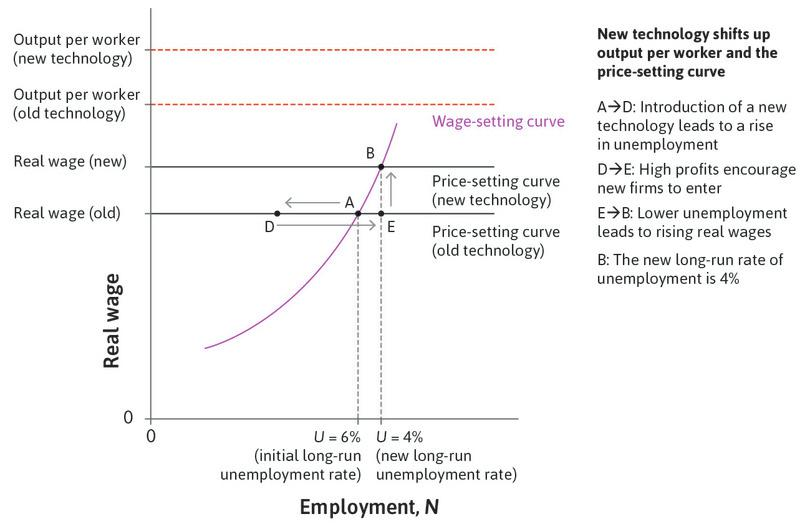
\includegraphics[width=\textwidth]{../QuestionBankImage/ECO-U16-Q7-01.jpg}
\answer{C}
\begin{tasks}(1)
    \task The new technology does not cause any increase in unemployment, either in the short run or in the long run.
        \details{In the short-run, initially there is a displacement of some workers from their jobs, which increases unemployment, as shown by the movement from point A to point D.}
    \task At D firms increase investment, and hence employment, due to the large gap between the real wage paid and the workers’ wage-setting curve.
        \details{Firms increase investment due to the large gap between the old real wage (solid line) and the new output per worker (dashed line), which implies higher profits.}
    \task Lower unemployment at E implies a higher wage required to induce workers to exert high effort, resulting in the higher real wage at B.
        \details{E is below the wage-setting curve so workers need a higher wage to be induced to work.}
    \task The adjustment from equilibrium A to the new equilibrium at B is immediate.
        \details{The adjustment to the new equilibrium requires entry of new firms, which can take a substantial amount of time.}
\end{tasks}




\Question (OUP-U16-Q6)
Last year, an economy had 1m registered unemployed and a labour force of 20m. Official statistics forecast a level of unemployment of 0.8m by the year’s end while the size of the labour force remains unchanged. If this happens then the unemployment rate will have:
\answer{B}
\begin{tasks}(1)
    \task Risen by 0.2m.
        \details{Incorrect. The level of unemployment has fallen by 0.2m. If the labour force is constant, then the rate of unemployment must also have fallen.}
    \task Fallen from 5 per cent to 4 per cent.
        \details{Correct. The unemployment rate has fallen from 1/20 (= 5\%) to 0.8/20 (= 4\%).}
    \task Fallen by 0.2m.
        \details{Incorrect. The level of unemployment has fallen by 0.2m, but the question asks about the rate.}
    \task Fallen by 0.2 per cent.
        \details{Incorrect. The level of unemployment has fallen by 0.2m but 0.2m is 1 per cent of 2m.}
\end{tasks}

\end{Exercise}

\end{document}
